\PassOptionsToPackage{unicode=true}{hyperref} % options for packages loaded elsewhere
\PassOptionsToPackage{hyphens}{url}
\documentclass[12pt,ignorenonframetext,compress]{beamer}
\IfFileExists{pgfpages.sty}{\usepackage{pgfpages}}{}
\setbeamertemplate{caption}[numbered]
\setbeamertemplate{caption label separator}{: }
\setbeamercolor{caption name}{fg=normal text.fg}
\beamertemplatenavigationsymbolsempty
\usepackage{lmodern}
\usepackage{amssymb}
\usepackage{amsmath}
\usepackage{ifxetex,ifluatex}
\usepackage{fixltx2e} % provides \textsubscript
\ifnum 0\ifxetex 1\fi\ifluatex 1\fi=0 % if pdftex
  \usepackage[T1]{fontenc}
  \usepackage[utf8]{inputenc}
\else % if luatex or xelatex
  \ifxetex
    \usepackage{mathspec}
  \else
    \usepackage{fontspec}
\fi
\defaultfontfeatures{Ligatures=TeX,Scale=MatchLowercase}






%
\fi

  \usetheme[]{iqss}






% use upquote if available, for straight quotes in verbatim environments
\IfFileExists{upquote.sty}{\usepackage{upquote}}{}
% use microtype if available
\IfFileExists{microtype.sty}{%
  \usepackage{microtype}
  \UseMicrotypeSet[protrusion]{basicmath} % disable protrusion for tt fonts
}{}


\newif\ifbibliography


\hypersetup{
      pdftitle={IQSS Beamer Class Demonstration},
        pdfauthor={Ista Zahn and Gary King},
          pdfborder={0 0 0},
    breaklinks=true}
%\urlstyle{same}  % Use monospace font for urls




  \usepackage{color}
  \usepackage{fancyvrb}
  \newcommand{\VerbBar}{|}
  \newcommand{\VERB}{\Verb[commandchars=\\\{\}]}
  \DefineVerbatimEnvironment{Highlighting}{Verbatim}{commandchars=\\\{\}}
  % Add ',fontsize=\small' for more characters per line
  \newenvironment{Shaded}{}{}
  \newcommand{\AlertTok}[1]{\textcolor[rgb]{1.00,0.00,0.00}{#1}}
  \newcommand{\AnnotationTok}[1]{\textcolor[rgb]{0.00,0.50,0.00}{#1}}
  \newcommand{\AttributeTok}[1]{#1}
  \newcommand{\BaseNTok}[1]{#1}
  \newcommand{\BuiltInTok}[1]{#1}
  \newcommand{\CharTok}[1]{\textcolor[rgb]{0.00,0.50,0.50}{#1}}
  \newcommand{\CommentTok}[1]{\textcolor[rgb]{0.00,0.50,0.00}{#1}}
  \newcommand{\CommentVarTok}[1]{\textcolor[rgb]{0.00,0.50,0.00}{#1}}
  \newcommand{\ConstantTok}[1]{#1}
  \newcommand{\ControlFlowTok}[1]{\textcolor[rgb]{0.00,0.00,1.00}{#1}}
  \newcommand{\DataTypeTok}[1]{#1}
  \newcommand{\DecValTok}[1]{#1}
  \newcommand{\DocumentationTok}[1]{\textcolor[rgb]{0.00,0.50,0.00}{#1}}
  \newcommand{\ErrorTok}[1]{\textcolor[rgb]{1.00,0.00,0.00}{\textbf{#1}}}
  \newcommand{\ExtensionTok}[1]{#1}
  \newcommand{\FloatTok}[1]{#1}
  \newcommand{\FunctionTok}[1]{#1}
  \newcommand{\ImportTok}[1]{#1}
  \newcommand{\InformationTok}[1]{\textcolor[rgb]{0.00,0.50,0.00}{#1}}
  \newcommand{\KeywordTok}[1]{\textcolor[rgb]{0.00,0.00,1.00}{#1}}
  \newcommand{\NormalTok}[1]{#1}
  \newcommand{\OperatorTok}[1]{#1}
  \newcommand{\OtherTok}[1]{\textcolor[rgb]{1.00,0.25,0.00}{#1}}
  \newcommand{\PreprocessorTok}[1]{\textcolor[rgb]{1.00,0.25,0.00}{#1}}
  \newcommand{\RegionMarkerTok}[1]{#1}
  \newcommand{\SpecialCharTok}[1]{\textcolor[rgb]{0.00,0.50,0.50}{#1}}
  \newcommand{\SpecialStringTok}[1]{\textcolor[rgb]{0.00,0.50,0.50}{#1}}
  \newcommand{\StringTok}[1]{\textcolor[rgb]{0.00,0.50,0.50}{#1}}
  \newcommand{\VariableTok}[1]{#1}
  \newcommand{\VerbatimStringTok}[1]{\textcolor[rgb]{0.00,0.50,0.50}{#1}}
  \newcommand{\WarningTok}[1]{\textcolor[rgb]{0.00,0.50,0.00}{\textbf{#1}}}

  \usepackage{longtable,booktabs}
  \usepackage{caption}
  % These lines are needed to make table captions work with longtable:
  \makeatletter
  \def\fnum@table{\tablename~\thetable}
  \makeatother

  \usepackage{graphicx,grffile}
  \makeatletter
  \def\maxwidth{\ifdim\Gin@nat@width>\linewidth\linewidth\else\Gin@nat@width\fi}
  \def\maxheight{\ifdim\Gin@nat@height>\textheight0.8\textheight\else\Gin@nat@height\fi}
  \makeatother
  % Scale images if necessary, so that they will not overflow the page
  % margins by default, and it is still possible to overwrite the defaults
  % using explicit options in \includegraphics[width, height, ...]{}
  \setkeys{Gin}{width=\maxwidth,height=\maxheight,keepaspectratio}

% Prevent slide breaks in the middle of a paragraph:
\widowpenalties 1 10000
\raggedbottom

  \AtBeginPart{
    \let\insertpartnumber\relax
    \let\partname\relax
    \frame{\partpage}
  }
  \AtBeginSection{
    \ifbibliography
    \else
      \let\insertsectionnumber\relax
      \let\sectionname\relax
      \frame{\sectionpage}
    \fi
  }
  \AtBeginSubsection{
    \let\insertsubsectionnumber\relax
    \let\subsectionname\relax
    \frame{\subsectionpage}
  }



\setlength{\parindent}{0pt}
\setlength{\parskip}{6pt plus 2pt minus 1pt}
\setlength{\emergencystretch}{3em}  % prevent overfull lines
\providecommand{\tightlist}{%
  \setlength{\itemsep}{0pt}\setlength{\parskip}{0pt}}

  \setcounter{secnumdepth}{0}



%% IQSS overrides
\iqsssectiontitle{Outline}

\AtBeginSection[]{
  \title{\insertsectionhead}
  {
    \definecolor{white}{rgb}{0.776,0.357,0.157}
    \definecolor{iqss@orange}{rgb}{1,1,1}
    \ifnum \insertmainframenumber > \insertframenumber
    \frame{
      \frametitle{\iqsssectiontitleheader}
      \tableofcontents[currentsection]
    }
    \else
    \frame{
      \frametitle{Backup Slides}
      \tableofcontents[sectionstyle=shaded/shaded,subsectionstyle=shaded/shaded/shaded]
    }
    \fi
  }
}

\AtBeginSubsection[]{}

%%


  \title[]{IQSS Beamer Class Demonstration}



  \author[
        Ista Zahn and Gary King
    ]{Ista Zahn and Gary King}

  \institute[
    ]{
    IQSS
    }

\date[
      \today
  ]{
      \today
        }

\begin{document}

% Hide progress bar and footline on titlepage
  \begin{frame}[plain]
  \titlepage
  \end{frame}



\hypertarget{beamer-features}{%
\section{Beamer Features}\label{beamer-features}}

\hypertarget{some-of-garys-examples}{%
\subsection{Some of Gary's Examples}\label{some-of-garys-examples}}

\begin{frame}{What's this course about?}
\protect\hypertarget{whats-this-course-about}{}

\begin{itemize}
\tightlist
\item
  \alert{Specific statistical methods for many research problems} - How
  to learn (or create) new methods - Inference:
  \underline{Using facts you know to learn about
        facts you don't know}
\item
  \alert{How to write a publishable scholarly paper}
\item
  \alert{All the practical tools of research} --- theory, applications,
  simulation, programming, word processing, plumbing, whatever is useful
\item
  \(\leadsto\) \alert{Outline and class materials:}

  \begin{itemize}
  \item
    \mbox{{\huge\parbox[b][.5in][t]{1in}{\alert{j.mp/G2001}}}
      $\qquad\qquad$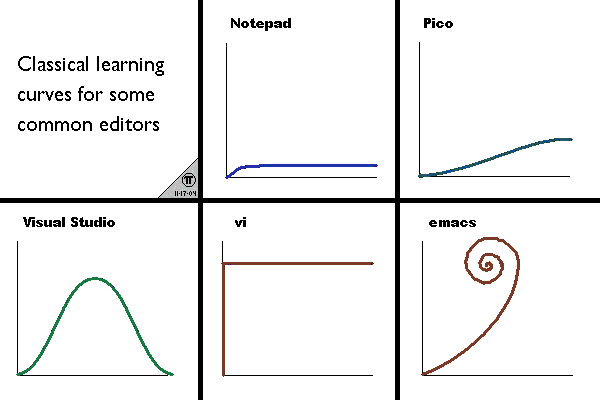
\includegraphics[width=.95in]{figs/phbAr.png}}
  \item
    The syllabus gives topics, not a weekly plan.
  \item
    We will go as fast as possible subject to everyone following along
  \item
    We cover different amounts of material each week
  \end{itemize}
\end{itemize}

\end{frame}

\begin{frame}{How much math will you scare us with?}
\protect\hypertarget{how-much-math-will-you-scare-us-with}{}

\begin{itemize}
\tightlist
\item
  All math requires two parts: \alertb{proof} and
  \alertb{concepts \& intuition}
\item
  Different classes emphasize:

  \begin{itemize}
  \tightlist
  \item
    \alert{Baby Stats}: dumbed down proofs, vague intuition
  \item
    \alert{Math Stats}: rigorous mathematical proofs
  \item
    \alert{\underline{Practical Stats}}: deep concepts and intuition,
    proofs when needed

    \begin{itemize}
    \tightlist
    \item
      Goal: how to do empirical research, in depth
    \item
      Use rigorous statistical theory --- when needed
    \item
      Insure we understand the intuition --- always
    \item
      Always traverse from theoretical foundations to practical
      applications
    \item
      Includes ``how to'' computation
    \item
      \(\leadsto\) Fewer proofs, more concepts, better practical
      knowledge
    \end{itemize}
  \end{itemize}
\item
  Do you have the background for this class? \alert{A Test: What's this?
    \begin{align*}
      b=(X'X)^{-1}X'y
    \end{align*} }
\end{itemize}

\end{frame}

\begin{frame}{Systematic Components: Examples}
\protect\hypertarget{systematic-components-examples}{}

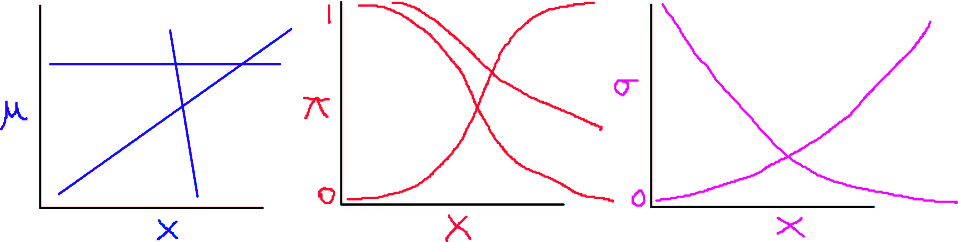
\includegraphics[width=8cm]{figs/functionalForms}

\begin{itemize}
\item
  \alertb{$E(Y_i) \equiv \mu_i = X_i\beta = \beta_0 +
      \beta_1X_{1i} +\dots+\beta_kX_{ki}$}
\item
  \alertc{$\Pr(Y_i=1) \equiv \pi_i =
      \frac{1}{1+e^{-x_i\beta}}$}
\item
  \alertd{$V(Y_i)\equiv \sigma_i^2 = e^{x_i\beta}$}
\item
  Interpretation:

  \begin{itemize}
  \tightlist
  \item
    Each is a \alert{class of functional forms}
  \item
    Set \(\beta\) and it picks out one \alert{member of the class}
  \item
    \alert{$\beta$} in each is an ``effect parameter'' vector, with
    different meaning
  \end{itemize}
\end{itemize}

\end{frame}

\begin{frame}[fragile]{Code blocks}
\protect\hypertarget{code-blocks}{}

\footnotesize

\begin{Shaded}
\begin{Highlighting}[]
\CommentTok{# Say hello in R}
\NormalTok{hello <-}\StringTok{ }\ControlFlowTok{function}\NormalTok{(name) }\KeywordTok{paste}\NormalTok{(}\StringTok{"hello"}\NormalTok{, name)}
\end{Highlighting}
\end{Shaded}

\begin{Shaded}
\begin{Highlighting}[]
\CommentTok{# Say hello in Python}
\KeywordTok{def}\NormalTok{ hello(name):}
\ControlFlowTok{return}\NormalTok{(}\StringTok{"Hello"} \OperatorTok{+} \StringTok{" "} \OperatorTok{+}\NormalTok{ name)}
\end{Highlighting}
\end{Shaded}

\begin{Shaded}
\begin{Highlighting}[]
\CommentTok{-- Say hello in Haskell}
\NormalTok{hello name }\FunctionTok{=} \StringTok{"Hello"} \FunctionTok{++} \StringTok{" "} \FunctionTok{++}\NormalTok{ name}
\end{Highlighting}
\end{Shaded}

```c /* Say hello in C */ \#include \textless{}stdio.h\textgreater{} int
main() \{ char name{[}256{]}; fgets(name, sizeof(name), stdin);
printf(``Hello \%s'', name); return(0); \}

\normalsize

\end{frame}

\begin{frame}{Alerts}
\protect\hypertarget{alerts}{}

\begin{itemize}
\tightlist
\item
  First level \alert{alert}
\item
  Second level \alertb{alert}
\item
  Third level \alertc{alert}
\item
  Fourth level \alertd{alert}
\item
  Fifth level \alerte{alert}
\end{itemize}

\end{frame}

\hypertarget{more-features}{%
\section{More Features}\label{more-features}}

\hypertarget{blocks}{%
\subsection{Blocks}\label{blocks}}

\begin{frame}{Other Features}
\protect\hypertarget{other-features}{}

\begin{block}{Levels of Structure}

\begin{itemize}
\tightlist
\item
  Clean, extensively customizable visual style
\item
  Hyperlinks
  (\href{click\%20here_}{http://github.com/izahn/iqss-beamer-theme}
\item
  No weird scaling prosper

  \begin{itemize}
  \tightlist
  \item
    slides are 96\textsubscript{mm}\(\times\)\textsubscript{128}mm
  \item
    text is 10-12pt on slide
  \item
    slide itself magnified with Adobe Reader/xpdf/gv to fill screen
  \end{itemize}
\item
  pgf graphics framework easy to use
\item
  include external JPEG/PNG/PDF figures
\item
  output directly to pdf: no PostScript hurdles
\item
  detailed User Manual (with good presentation advice, too)
\end{itemize}

\end{block}

\end{frame}

\begin{frame}{Theorems and Proofs}
\protect\hypertarget{theorems-and-proofs}{}

\framesubtitle{The proof uses \textit{reductio ad absurdum}.}

\begin{block}{Theorem}

There is no largest prime number.

\end{block}

\begin{block}{Proof}

\begin{itemize}[<+->]
\tightlist
\item
  Suppose \(p\) were the largest prime number.
\item
  Let \(q\) be the product of the first \(p\) numbers.
\item
  Then \(q+1\) is not divisible by any of them.
\item
  But \(q + 1\) is greater than \(1\), thus divisible by some prime
  number not in the first \(p\) numbers. \qedhere
\end{itemize}

\end{block}

\end{frame}

\begin{frame}{Blocks}
\protect\hypertarget{blocks-1}{}

\begin{block}{Normal block}

A \alert{set} consists of elements.

\end{block}

\begin{block}{\alert{Alert block}}

\(2=2\).

\end{block}

\begin{block}{\alertc{Example block}}

The set \(\{1,2,3,5\}\) has four elements.

\end{block}

\end{frame}

\hypertarget{rmarkdown-examples}{%
\section{RMarkdown Examples}\label{rmarkdown-examples}}

\begin{frame}[fragile]{R Figure}
\protect\hypertarget{r-figure}{}

The following code generates the plot on the next slide (taken from
\texttt{help(bxp)} and modified slightly):

\begin{Shaded}
\begin{Highlighting}[]
\KeywordTok{library}\NormalTok{(stats)}
\KeywordTok{set.seed}\NormalTok{(}\DecValTok{753}\NormalTok{)}
\NormalTok{bx.p <-}\StringTok{ }\KeywordTok{boxplot}\NormalTok{(}\KeywordTok{split}\NormalTok{(}\KeywordTok{rt}\NormalTok{(}\DecValTok{100}\NormalTok{, }\DecValTok{4}\NormalTok{),}
                      \KeywordTok{gl}\NormalTok{(}\DecValTok{5}\NormalTok{, }\DecValTok{20}\NormalTok{)), }\DataTypeTok{plot=}\OtherTok{FALSE}\NormalTok{)}
\KeywordTok{bxp}\NormalTok{(bx.p, }\DataTypeTok{notch =} \OtherTok{FALSE}\NormalTok{, }\DataTypeTok{boxfill =} \StringTok{"lightblue"}\NormalTok{,}
    \DataTypeTok{frame =} \OtherTok{FALSE}\NormalTok{, }\DataTypeTok{outl =} \OtherTok{TRUE}\NormalTok{,}
    \DataTypeTok{main =} \StringTok{"Example from help(bxp)"}\NormalTok{)}
\end{Highlighting}
\end{Shaded}

\end{frame}

\begin{frame}{R Figure}
\protect\hypertarget{r-figure-1}{}

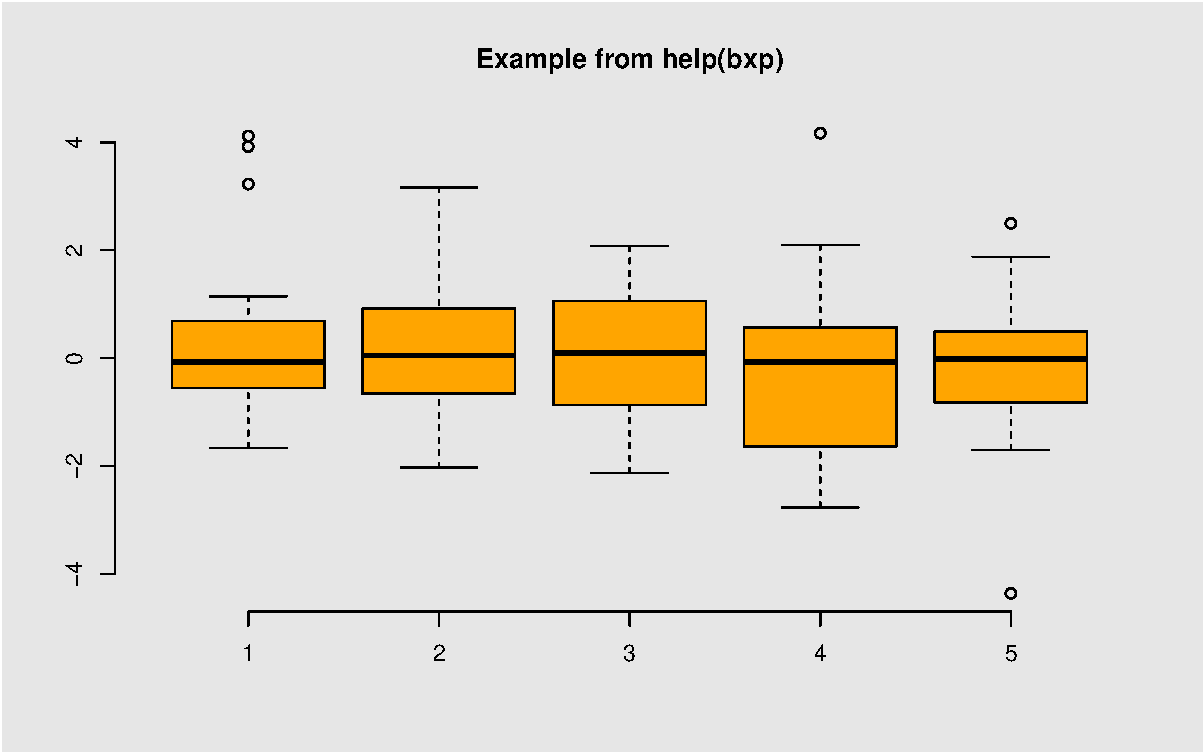
\includegraphics{beamer_template_iqss_files/figure-beamer/pressureFig-1.pdf}

\end{frame}

\begin{frame}[fragile]{R Table}
\protect\hypertarget{r-table}{}

A simple \texttt{knitr::kable} example:

\small

\begin{Shaded}
\begin{Highlighting}[]
\NormalTok{knitr}\OperatorTok{::}\KeywordTok{kable}\NormalTok{(mtcars[}\DecValTok{1}\OperatorTok{:}\DecValTok{5}\NormalTok{, }\DecValTok{1}\OperatorTok{:}\DecValTok{8}\NormalTok{],}
             \DataTypeTok{caption=}\StringTok{"(Parts of) the mtcars dataset"}\NormalTok{)}
\end{Highlighting}
\end{Shaded}

\begin{longtable}[]{@{}lrrrrrrrr@{}}
\caption{(Parts of) the mtcars dataset}\tabularnewline
\toprule
& mpg & cyl & disp & hp & drat & wt & qsec & vs\tabularnewline
\midrule
\endfirsthead
\toprule
& mpg & cyl & disp & hp & drat & wt & qsec & vs\tabularnewline
\midrule
\endhead
Mazda RX4 & 21.0 & 6 & 160 & 110 & 3.90 & 2.620 & 16.46 &
0\tabularnewline
Mazda RX4 Wag & 21.0 & 6 & 160 & 110 & 3.90 & 2.875 & 17.02 &
0\tabularnewline
Datsun 710 & 22.8 & 4 & 108 & 93 & 3.85 & 2.320 & 18.61 &
1\tabularnewline
Hornet 4 Drive & 21.4 & 6 & 258 & 110 & 3.08 & 3.215 & 19.44 &
1\tabularnewline
Hornet Sportabout & 18.7 & 8 & 360 & 175 & 3.15 & 3.440 & 17.02 &
0\tabularnewline
\bottomrule
\end{longtable}

\end{frame}

\begin{frame}{Resources}
\protect\hypertarget{resources}{}

\begin{block}{For more information:}

\begin{itemize}
\tightlist
\item
  See the \href{https://github.com/IQSS/iqss-beamer-theme}{IQSS
  repository} for more on the IQSS them
\item
  See the \href{https://github.com/rstudio/rmarkdown}{RMarkdown
  repository} for more on RMarkdown
\item
  See the \href{https://github.com/eddelbuettel/binb}{binb repository}
  for more on binb
\item
  See the \href{https://github.com/eddelbuettel/binb/vignettes}{binb
  vignettes} for more examples.
\end{itemize}

\end{block}

\end{frame}




\end{document}
